\documentclass[draft,final]{thesisclass} % Remove option 'final' to obtain debug information.

% Load packages to allow in- and output of non-ASCII characters.
\usepackage{lmodern}        % Use an extension of the original Computer Modern font to minimize the use of bitmapped letters.
\usepackage[T1]{fontenc}    % Determines font encoding of the output. Font packages have to be included before this line.
\usepackage[utf8]{inputenc} % Determines encoding of the input. All input files have to use UTF8 encoding.

% added package for bibliography
\usepackage{csquotes}
\usepackage[backend=biber,style=authoryear,date=year,maxbibnames=10,dashed=false]{biblatex}
\addbibresource{thesis.bib}
\DeclareDelimFormat[bib,biblist]{nametitledelim}{\addcolon\space}
\DeclareDelimFormat{postnotedelim}{\addcolon\space}

% for definitions
\usepackage{amsthm}
\newtheorem{definition}{Definition}

% Extended LaTeX functionality is enables by including packages with \usepackage{...}.
\usepackage{amsmath}    % Extended typesetting of mathematical expression.
\usepackage{amssymb}    % Provides a multitude of mathematical symbols.
\usepackage{mathtools}  % Further extensions of mathematical typesetting.
\usepackage{microtype}  % Small-scale typographic enhancements.
\usepackage[inline]{enumitem} % User control over the layout of lists (itemize, enumerate, description).
\usepackage{multirow}   % Allows table elements to span several rows.
\usepackage{booktabs}   % Improves the typesetting of tables.
\usepackage{subcaption} % Allows the use of subfigures and enables their referencing.
\usepackage[ruled,linesnumbered,algochapter]{algorithm2e} % Enables the writing of pseudo code.
\usepackage[usenames,dvipsnames,table]{xcolor} % Allows the definition and use of colors. This package has to be included before tikz.
\usepackage{nag}       % Issues warnings when best practices in writing LaTeX documents are violated.
\usepackage{todonotes} % Provides tooltip-like todo notes.
\usepackage{hyperref}  % Enables hyperlinking in the electronic document version. This package has to be included second to last.
\usepackage[acronym,toc]{glossaries} % Enables the generation of glossaries and lists of acronyms. This package has to be included last.
\usepackage{lipsum}  % Provides blind text.
\usepackage{acronym} % Provides a list of acronyms.
\usepackage{float} % Provides the H float modifier option.
\usepackage{tabularx} % Provides a tabular package.
\usepackage{listings} % for code listings.

% Define convenience functions to use the author name and the thesis title in the PDF document properties.
\newcommand{\authorname}{Hannes Brantner} % The author name without titles.
\newcommand{\thesistitle}{Enhancing recruitment efficiency by exploring the impact of large language models on the screening process} % The title of the thesis. The English version should be used, if it exists.

% Set PDF document properties
\hypersetup{
    pdfpagelayout   = TwoPageRight,           % How the document is shown in PDF viewers (optional).
    linkbordercolor = {Melon},                % The color of the borders of boxes around hyperlinks (optional).
    pdfauthor       = {\authorname},          % The author's name in the document properties (optional).
    pdftitle        = {\thesistitle},         % The document's title in the document properties (optional).
    pdfsubject      = {LLMs in \acs{HR}},              % The document's subject in the document properties (optional).
    pdfkeywords     = {Machine Learning, \acs{HR}, Human Resources, \acs{AI}, LLM} % The document's keywords in the document properties (optional).
}

\setpnumwidth{2.5em}        % Avoid overfull hboxes in the table of contents (see memoir manual).
\setsecnumdepth{subsection} % Enumerate subsections.

\nonzeroparskip             % Create space between paragraphs (optional).
\setlength{\parindent}{0pt} % Remove paragraph indentation (optional).

\makeindex      % Use an optional index.
\makeglossaries % Use an optional glossary.
%\glstocfalse   % Remove the glossaries from the table of contents.

% Set persons with 4 arguments:
%  {title before name}{name}{title after name}{gender}
%  where both titles are optional (i.e. can be given as empty brackets {}).
\setauthor{Ing. Dipl.-Ing.}{\authorname}{}{male}
\setadvisor{Mag. Dr.}{Alexander Pfeiffer}{MBA MA}{male}

% For bachelor and master theses:
\setfirstassistant{}{Michaela Wawra}{MSc}{female}
% \setsecondassistant{Pretitle}{Forename Surname}{Posttitle}{male}
% \setthirdassistant{Pretitle}{Forename Surname}{Posttitle}{male}

% For dissertations:
% \setfirstreviewer{Pretitle}{Forename Surname}{Posttitle}{male}
% \setsecondreviewer{Pretitle}{Forename Surname}{Posttitle}{male}

% For dissertations at the PhD School and optionally for dissertations:
% \setsecondadvisor{Pretitle}{Forename Surname}{Posttitle}{male} % Comment to remove.

% Required data.
\setregnumber{01614466}
\setdate{01}{10}{2023} % Set date with 3 arguments: {day}{month}{year}.
\settitle{\thesistitle}{\thesistitle} % Sets English and German version of the title (both can be English or German). If your title contains commas, enclose it with additional curvy brackets (i.e., {{your title}}) or define it as a macro as done with \thesistitle.
\setsubtitle{}{} % Sets English and German version of the subtitle (both can be English or German).

% Select the thesis type: bachelor / master / doctor.
% Bachelor:
% \setthesis{bachelor}
%
% Master:
\setthesis{master}
\setmasterdegree{master} % dipl. / rer.nat. / rer.soc.oec. / master
%
% Doctor:
%\setthesis{doctor}
%\setdoctordegree{rer.soc.oec.}% rer.nat. / techn. / rer.soc.oec.

% For bachelor and master:
\setcurriculum{Master in Business Administration (One Year MBA)}{Master in Business Administration (One Year MBA)} % Sets the English and German name of the curriculum.

% Optional reviewer data:
\setfirstreviewerdata{Affiliation, Country}
\setsecondreviewerdata{Affiliation, Country}

% Add glossary entries.
\newglossaryentry{LLM}
{
    name=Large Language Model,
    description={A Large Language Model is reading and emitting text, enabling it to perform tasks such as translation, summarization, and question answering}
}
\newglossaryentry{TTH}
{
    name=time-to-hire,
    description={The time from the receiving of the candidate's application to the accepted job offer}
}
\newglossaryentry{TAPJFNN}{
    name=Topic-Based Ability-Aware Person-Job Fit Neural Network,
    description={This framework based on the Recurrent Neural Network architecture for predicting person-job fit was introduced in \textcite{pj_fit_ml}}
}

% define style for Javascript scripts
\lstdefinelanguage{TypeScript}{
  keywords={typeof, new, true, false, catch, function, return, null, catch, switch, var, if, in, while, do, else, case, break},
  keywordstyle=\color{blue}\bfseries,
  ndkeywords={class, export, boolean, throw, implements, import, this},
  ndkeywordstyle=\color{darkgray}\bfseries,
  identifierstyle=\color{black},
  sensitive=false,
  comment=[l]{//},
  morecomment=[s]{/*}{*/},
  commentstyle=\color{purple}\ttfamily,
  stringstyle=\color{red}\ttfamily,
  morestring=[b]',
  morestring=[b]"
}
\lstset{
  basicstyle=\ttfamily,
  columns=fullflexible,
  frame=single,
  breaklines=true,
  postbreak=\mbox{\textcolor{red}{$\hookrightarrow$}\space},
  captionpos=b,
}

\begin{document}

\frontmatter % Switches to roman numbering.
% The structure of the thesis has to conform to the guidelines at
%  https://informatics.tuwien.ac.at/study-services

% \addtitlepage{naustrian} % German title page.
\addstatementpage
\addtitlepage{english} % English title page.

% citation tutorial
% cite only page 1
% \parencite[1]{discrimination_algorithms} \newline
% cite page 2 to 5
% \parencite[2-5]{discrimination_algorithms} \newline
% cite page 3 and the following page
% \parencite[3f]{discrimination_algorithms} \newline
% cite page 3 and the following pages
% \parencite[3ff]{discrimination_algorithms} \newline

\begin{acknowledgements}
\lipsum[1]
\end{acknowledgements}

% Use an optional list of figures.
\listoffigures % Starred version, i.e., \listoffigures*, removes the toc entry.
\cleardoublepage

% Use an optional list of tables.
\listoftables % Starred version, i.e., \listoftables*, removes the toc entry.
\cleardoublepage

\chapter{List of Abbreviations}
% Add acronym entries.
\begin{acronym}
    \acro{AI}{Artificial Intelligence}
    \acro{CV}{Curriculum Vitae}
    \acro{LLM}{Large Language Model}
    \acro{HR}{Human Resources}
    \acro{NLP}{Natural Language Processing}
    \acro{TAPJFNN}{Topic-Based Ability-Aware Person-Job Fit Neural Network}
\end{acronym}
\cleardoublepage

% Select the language of the thesis, e.g., english or naustrian.
\selectlanguage{english}

% Add a table of contents (toc).
\tableofcontents % Starred version, i.e., \tableofcontents*, removes the self-entry.

\chapter{Executive Summary}
\lipsum[1]
\cleardoublepage

\begin{abstract}
\lipsum[1]
\end{abstract}

% Switch to arabic numbering and start the enumeration of chapters in the table of content.
\mainmatter

\chapter{Introduction} \label{introduction}

\section{Problem Statement} \label{problem_statement}
This section relies heavily on the article \textcite{ai_recruiting} which is based on over $50$ research papers in that field and which describes the evolution of the recruiting in a very concise way.
As described in \textcite[1]{ai_recruiting}, the average firm's value by 2000 was roughly consisting of 65\% of value from intangible assets.
This has evolved a lot, as by the end of 1980, around 70 to 90\% of tangible assets were accountable for the average firm's value \parencite[1]{ai_recruiting}.
This means that the value of a firm is more and more dependent on the quality of its employees and the knowledge they possess and this ongoing process does not seem to come to a halt in the near future.
The technological context of how companies recruit people has also evolved a lot over the last decades, as machine learning tools are more and more used to automate processes or assist humans in attracting the right candidates, screening, assessing and selecting them \parencite[2]{ai_recruiting}.
The article \textcite[2-4]{ai_recruiting} described four evolution stages of recruiting which are the following:
\begin{enumerate}
    \item \textbf{Analog Recruiting} \label{analog_recruting}\\
    The first stage is the analog recruiting stage where people were the main mechanism of recruiting new employees.
    Prospective applicants needed to go to the company to manually turn a paper job application in.
    Companies want to maximize the information richness they supply for the current job vacancy but also the information reach to attract as many promising applicants as possible.
    But as described in \textcite[2]{ai_recruiting}, in analog recruiting these two goals faced the analog reach and richness frontier as shown in \ref{fig:analog_reach_richness_frontier} because the more information is supplied, the more costly it is when you supply to media with great reach at that time:
    \begin{figure}[H]
        \centering
        \includegraphics[scale=0.5,page=2,width=0.6\linewidth,trim={300 100 55 515},clip]{literature/ai_recruiting.pdf}
        \caption{Analog reach and richness frontier \parencite[2]{ai_recruiting}}
        \label{fig:analog_reach_richness_frontier}
    \end{figure}
    \item \textbf{Digital Recruiting 1.0} \label{digital_recruiting_1}\\
    This first evolution stage of digital recruiting that happened in the late 1990s was characterized by breaking the analog reach and richness frontier by using digital media which allowed to supply rich information to many prospective candidates at a very low cost because there were no printing and low distribution costs involved.
    There was also a change on the applicant's side as no more manually filled out documents were required to be handed in physically at the company site.
    It also allowed them filter out job offers based on various selectors and it also allowed companies to offer more dynamic content to the job seekers by adding video and audio data to the job search websites.
    There was also a considerable exponential and self-enforcing network effect that was ongoing at that time for job search websites \parencite[3]{ai_recruiting}.
    As they listed more and more job offers, more and more job seekers were attracted to the platform which made it easier to persuade companies to list their job offers on the job search websites.
    \item \textbf{Digital Recruiting 2.0} \label{digital_recruiting_2}\\
    This evolution step emerged around ten years after the first evolution of Digital Recruiting and was mainly driven by two developments.
    The first development was the rise of job board aggregation services that presented all job offers from various job search websites on one platform.
    Job seekers now have access to all available job offers without having to visit each platform individually and job firms do not need to publish their offer at each individual website.
    The second development was the introduction and rise of professional social network platforms such as \textit{LinkedIn}.
    These network platforms allowed people to form professional communities and groups of interest and also allowed companies to present themselves to the public and to potential applicants.
    Moreover, with endorsements people in such platforms could endorse skills of others which allowed to build a reputation and trust in the community.
    It enabled companies to target their job ads more effectively to promising candidates, contact candidates directly through the network and also enabled a cheap and efficient way to post job offers on large social websites whether they are professional or not like \textit{Facebook} \parencite[3]{ai_recruiting}.
    \item \textbf{Digital Recruiting 3.0} \label{digital_recruiting_3}\\
    After Digital Recruiting matured from 2010 to 2015, Digital Recruiting 3.0 emerged and was primarily driven by the rise of machine learning and artificial intelligence in human resources processes.
    As digital recruiting digitized the processes and also made the processes more frictionless for employers and employees, more and more applications came in for each job offer, on average the number is around 250 applications per job offer \parencite[4]{ai_recruiting}. 
    This can be explained by the fact that the cost of applying is very low for the applicant, but this led to about 80\% of the applications being unqualified \parencite[4]{ai_recruiting}.
    To deal with this massive amount of applicants, you can either deploy more human resources to screen the applications or you can use machine learning to either automate processes or assist humans such that they can work more productively.
    Human Resources are mission-critical for companies as the human capital is getting more and more important for the success of a company.
    Moreover, research showed that top performers are four to eight times more productive that the average performers, increasingly so in complex environments, according to \textcite[4]{ai_recruiting}.
    Furthermore, this new evolution stage of recruiting also has its downsides as discussed in \textcite[4-5]{challenges_opportunities_hr} due to the emerging use of technology:
    \begin{itemize}
        \item It was stated that the use of technology in human resources typically leads to more efficiency and decreasing costs associated to human resources transactions, but some researchers argue that there is no considerable effect on the main goal of human resources to attract, motivate and maintain talented employees. 
        \item Furthermore, it is argued that the used technologies are often static and one-way communication systems that do not allow either side of the recruiting process to ask questions. This may entail creating an artificial distance between the applicant and the people doing the recruitment tasks. The technologies of the future which are already here, are already capable of partially mitigating those drawbacks.
        \item The article also discussed that if the tasks of complete human resource departments are transferred to other employees and managers, this may have a negative effect on the overall productivity of organizations. This also means that if the administrative burden for the human resource department is reduced, it can also contribute to the strategic direction of organizations.
    \end{itemize}
    More consideration on the use of \acs{AI}-assisted technologies regarding recruiting are presented here \parencite[2-4]{ai_in_hr_management}:
    \begin{itemize}
        \item Algorithms that help filtering applicants and were trained with imitation learning are often trained with biased data. As these algorithms try to map input attributes or features to desirable outputs like job performance present in the training data sets, it keeps the bias from past recruiting activities like hiring less women in top management positions in favor for men. Also \textit{Amazon} had this bias problem in their hiring algorithm which is an alarming sign for the use of \acs{AI} in human resources due to legal considerations and violations of the social norms.
        \item Furthermore, as applicants more and more discover the biases of the used algorithms or traits that they will like, applicants may more and more artificially craft applications documents to meet the algorithm's expectations.
        \item The article also discussed that it is hard to define what a \textit{good employee} actually is. Most sources define a good employee based on performance appraisal scores, but those are very hard to measure as any reasonably complex job is interdependent with other jobs, making it very hard to disentangle the individual performance from the group performance. The performance metrics are often criticized for a lack of validity and reliability while having a considerable bias. Therefore, it is very hard and nearly impossible to achieve exactly this behavior of selecting high-performant applicants with imitation learning and unsuitable training data.
        \item Algorithms based on imitation learning require large amounts of past data and important events like dismissals may be sparse in the training data.
        \item Moreover, algorithms are not liable for their decisions, even though  hiring activities have a huge effect and the organization dynamics. Most algorithms in use today lack the capability to explain what attributes have actually driven the final decision.
    \end{itemize}
\end{enumerate}
This should have made the need for an effective human resources pipeline clear. To improve this pipeline machine learning tools are deployed to the following four fields \parencite[4-8]{ai_recruiting}:
\begin{enumerate}
    \item \textbf{Outreach}\\
    Firms try to identify candidates and get job opportunities in front of them in a way that invites them to
    actually apply. Machine learning can help to refine the job description in ways to attract more applicants or to bring more balance to the gender of the applicants. As there are more passive candidates not actively searching for a job than actively searching candidates, machine learning can be used to identify suitable talents from a massive pool of candidates, e.g. hundreds of millions of \textit{LinkedIn} users.
    \item \textbf{Screening}\\
    This stage should pre-filter the applicants to only keep the most promising ones for the next assessment stage.
    As stated in \textcite[6]{ai_recruiting}, machine learning tools were at least 25\% superior to humans even when they got a reasonable amount of time to screen the application. Furthermore, the \acs{AI}-enabled screening tool provider \textit{Ideal} says that with its technology the average \gls{TTH} fell from 24 days to 9 days.
    Moreover, \textit{L'Oréal} reported a drop of screening time per resume from 40 minutes to 4 minutes and \textit{Hilton Hotels \& Resorts} reported a drop of \gls{TTH} from 42 days to 5 days by incorporating \acs{AI} tools in the recruitment process.
    \item \textbf{Assessment}\\
    The assessments typically involve one to many rounds of assessment to determine the best or most suitable candidates that then will receive a job offer. Recent research showed that gamification with short games is more and more used to measure certain personality traits of candidates like risk aversion. Companies like \textit{Unilever} and \textit{L'Oréal} used \acs{AI}-chatbots that asked various questions and applicants were able to record video responses in the \textit{Unilever} case and chat response in the case of \textit{L'Oréal}. The \acs{AI} systems analyzed the content, the word choice and the used structure and matched the responses against successful employees in that field. In the case of video content, the system can also analyze the tone of the voice and the micro-facial movements. These two chatbots could be filled with information at any time within the given timeframe, so it reduces scheduling times with candidates and also gives candidates more freedom to answer the questions at a time that suits them best. These chatbots can also be used to fill in missing information from the job seekers like potential start date and can also answer questions regarding the salary range for example.
    \item \textbf{Coordination}\\
    This task contains the coordination with the applicants which involves appointment scheduling and appointment cancellation. As in the age of digital recruitment more and more candidates are rejected, and therefore you need to make sure to convey this information to all of your applicants, as little to no information regarding the process is the main driver for bad experiences with the application process. Machine learning tools can help to achieve that.
\end{enumerate}
By 2018 only around 40\% have used machine learning tools in these four core human resource sourcing processes \parencite[4]{ai_recruiting}.
The cost to implement, to integrate and to maintain \acs{AI} tools in human resources is significant and most companies should use services from external providers if they do not have massive amounts of hires to amortize these costs \parencite[8]{ai_recruiting}.
Furthermore, if the \acs{AI} tools are not used as an assistive technology, but as a technology to replace humans in the human resource sector, the acceptance of these technologies within this sector is quite low \parencite[9]{ai_recruiting}.
Moreover, around 70\% of large organization change initiatives which also include digital transformations, fail.
That means there is some space for improvement and this thesis tries to implement a new open-source tool in the area of screening to improve the productivity of the human resources workers in companies of any size.
As \acs{LLM}s are capable of summarization and question-answering when they are presented natural text as input within their context length, the problem to solve now is to match a provided \acs{CV} from an applicant to the applied job description and assign this match a score.
Furthermore, the model should also characterize the applicant as promising or not using an additional output.
The score should represent the suitability of the candidate for the job description and is needed to easily compare candidates and to sort them by their score.

\section{Significance of the Work} \label{significance_of_the_work}
The advantages of Digital Recruiting 3.0 should be available to all companies and not just to big corporations or as paid services from external providers.
The usage of machine learning tools should also not have the preconditions to have massive datasets in order to train and use the models.
Usage of the model should bring efficiency benefits without needing to use it lots of times in order to amortize the costs, making it perfectly viable for small companies.

\section{Research Objective and Research Question} \label{research_objective_and_research_question}
The research objective is to supply the proposed reasonably accurate screening tool based on \acs{LLM}s that was outlined in \ref{problem_statement} as open-source software to the public. 
That means companies of any size can use this tool and integrate it to their human capital sourcing pipelines to eventually increase their efficiency and decrease costs.
As outlined in the previous chapters, people working in human resources have to screen more and more resumes or \acs{CV}s as the reach of online job advertisements attracts many applicants.
It was also discussed that many of these applicants are not qualified enough for the advertised job and should therefore not be assessed further.
This pre-filtering saves costly human resources and makes it easier to invest the most time and effort into the most promising candidates, given that you have an easy and cheap way to screen the application documents.
With the rise of \acs{LLM}s which are capable of summarization and question answering, the idea was born to use these capabilities and apply them to the screening task in human resources.
\\\\
The research question is:\\
\textit{What impact could such an \acs{LLM}-based screening model have on the screening process?}\\\\
This formulation entails subordinate research questions which are shown in the following enumeration:
\begin{itemize}
    \item \textit{What is the accuracy of the proposed model?}\\
    This question will be answered by testing the accuracy of the model's outputs against annotations from human expert recruiters.
    This procedure is described in detail in \ref{quantitative_research_design}.
    \item \textit{What are the time savings associated to the model usage?}\\
    This question will be answered by measuring the time taken by the human experts to execute the above-mentioned data annotation.
    This time will be compared to a sampled time it takes for users to automate the same tasks using the model.
\end{itemize}

\section{Research Methodology} \label{research_methodology}
This thesis uses qualitative research design \ref{qualitative_research_design} and quantitative research design \ref{quantitative_research_design} to answer the research question.
In the qualitative context, the current state of experiences with and expectations from \acs{AI}-assisted tooling will be explored by a discussion with human experts in the human resources field.
In the quantitative context, the accuracy of the proposed model will be measured and the time savings associated to the model usage will be measured by comparing the model's statistics against the results from human expert recruiters.

\section{Structure of the Work} \label{structure_of_the_work}
This thesis starts with the introduction chapter \ref{introduction} which gives an overview of the problem statement \ref{problem_statement}, the significance of the work \ref{significance_of_the_work}, the research objective and research question \ref{research_objective_and_research_question}, the research methodology \ref{research_methodology} and the structure of the work \ref{structure_of_the_work}.
The second chapter \ref{theoretical_background} gives an overview of the theoretical background of the work, like quickly revisiting \gls{LLM}s and then discussing literature on person-environment fit and methods how to quantize this fit.
Afterwards, the methodology chapter \ref{methodology} describes what research methods have been used, how the results have been obtained and how to sample screening documents and the model have been created.


\chapter{Theoretical Background} \label{theoretical_background}

\section{Large Language Models}
The machine learning model type \gls{LLM} is commonly abbreviated as \acs{LLM} and makes natural language texts processable for computers.
The model works by compressing the read text into an internal state and based on this state an output text is generated.
As the model compresses the data according to the learned patterns in the training data, it does not understand the text in the same way as humans do.
These models are used to perform tasks such as translation, summarization, and question answering \parencite[1]{llm_literature_review}.
As this enabled a wide field of automation for application fields that were primarily carried out by humans, many technology companies have developed their own \acs{LLM} and made their services available to the public while keeping their source code mostly private.
Some notable example are the PaLM 2 model by Google \parencite{palm2} that powers Bard, the GPT-4 model by OpenAI \parencite{gpt4} that powers ChatGPT and the Llama 2 model by Meta \parencite{llama2}.
The Llama 2 model is the only model from the picked three candidates that has been released with public source code.
That means that researches and engineers around the world can use the model as building block and either improve the underlying mechanisms or try to incorporate it in their own applications.
The real breakthrough of \acs{LLM}s came with the release of the GPT-3 model by OpenAI \parencite{gpt3} that powered the initial version of ChatGPT.
They offered the model's capabilities as a website that was accessible to the public and allowed users to insert text and receive a response from the model.
As described in \textcite[1]{gpt3}, the model provided very good performance on various \acs{NLP} datasets that include tasks like translation and question answering.
To briefly visualize the complexity behind a \acs{LLM}, consider the function $f_{a,b,c}(x) = ax^2+bx+c$ that has the three parameters $a$, $b$ and $c$.
Here, the function $f$ maps the input data denoted as $x$ to the output data denoted as $f(x)$.
The input data in the \acs{NLP} case is the input text and the output data is the output text.
\acs{LLM}s also make use of parameterized and differentiable functions in their internal structure to map the input text to the output text, but they have orders of magnitudes more parameters than this sample function.
For example, the model GPT-3 uses 175 billion parameters \parencite[1]{gpt3} in total. The parameter count of GPT-4 was not disclosed in their technical report \parencite{gpt4}.
The training data needed to train these models was present in the required amounts because the researchers have not used reinforcement learning \parencite{rl_bible} or supervised learning \parencite[3]{sl_bible}.
Reinforcement learning gives the model a reward when an action was good and a punishment when an action was bad, this can be done by letting the model train in the real world which has bad scalability or in simulators that must be coded to mimic the real world which is also a very difficult and time consuming task.
For example, animals learn that behaviors that lead to food are good and behaviors that lead to hunger are bad.
The supervised learning approach labels input data with the desired output label and based on these mappings and a huge amount of training samples, the model will adjust its parameters to map the input data correctly.
An example would be input images that would be labeled with the object that can be seen on the images. So each input image must be labeled by hand before the model can be trained to predict it itself correctly.
To compress the patterns in the training data and fill them into the model parameters, huge amounts of training data are needed as the parameter count of \acs{LLM}s is huge.
Both techniques were not sufficient to train models of that sheer size, so the researchers used a technique called self-supervised learning \parencite[7]{llm_literature_review} where the model tries to fill in artificially generated gaps in the text.
Because the gaps are artificially introduced, the expected output is known in advance, so the model can be trained without the need of labeled training data which makes this technique very scalable.
Before the text is fed to the model it is tokenized \parencite[4]{llm_literature_review}, that means the text is converted into a sequence of tokens which can either be symbols, characters, subwords and words.
The model gets the tokenized text input and predicts the follow-up output tokens that will likely follow these input tokens. The output tokens are converted back into text and then the text from the artificial gap is compared to the model output.
Based on this comparison, the model parameters are adjusted. As no human data labelling or costly real-world or simulator training is needed, the model can be trained on huge amounts of data.
Most of the text data used for training large language models is scraped from the internet \parencite[1]{llm_literature_review}.
The context size of a \acs{LLM} is the number of tokens that the model can store in its internal state while generating the output tokens, so it is the history of tokens it can access while generating the response.
For example, the context size of the Llama 2 model is 4096 tokens \parencite[47]{llama2}.
The tokenizer that OpenAI is using, can be accessed via this website \textcite{openai_tokenizer}.
The output tokens of a \acs{LLM} are generated token by token, so when the first token is generated, it is appended to the input and the model generates the next token based on the input that now contains the first generated token. Afterwards, it is run iteratively in the same way.
That means that the total output token size is also constrained by the context size, when the full history of tokens should be within the context size while generating the output.
The model stops the output loop, when the model emits the stop token. That means that it has finished the output token generation.
Most of \acs{LLM}s are based on the machine learning model type called Transformers \parencite[1]{transformer} which is a neural network architecture that is based on the attention mechanism.

\section{Person-Environment Fit}
The person-environment fit can be broken up into the person-organization and the person-job fit.
For this section lots of citations are made from the article \textcite{po_and_pj_fit_literature_review} as it is a very good summary of more than $90$ research papers in this field.
Person-organization fit describes the compatibility between the applicant's and the organization's values and characteristics and how good they meet each other's needs \parencite[179]{po_and_pj_fit_literature_review}.
The person-job fit describes the compatibility between the applicant's abilities and the job's demands or the person's desires and the job's attributes \parencite[179]{po_and_pj_fit_literature_review}.
These two fit measures should both be considered when computing the score.

\subsection{Person-Environment Fit Types} \label{pef_types}
In essence, person-environment fit is a complex and multi-dimensional concept.
It can be conceptualized as both complementary and supplementary. 
Supplementary fit happens when a person supplements, embellishes or possesses characteristics that are similar to other individuals in the environment \parencite[180]{po_and_pj_fit_literature_review}.
Complementary fit happens when a person possesses characteristics that are missing in the environment and make it more complete \parencite[180]{po_and_pj_fit_literature_review}.
Complementary person-environment fit encompasses the needs-supplies and demands-abilities perspectives. 
A environment supplies financial, physical and psychological resources as well as task-related, interpersonal and growth opportunities that are demanded or needed by the person \parencite[180]{po_and_pj_fit_literature_review}.
When the supply meets the individual's needs, a needs-supplies fit is achieved.
A demands-abilities fit is achieved when the individual's professional contributions in terms of time, effort, commitment, skills and knowledge meet the demands of the environment \parencite[180]{po_and_pj_fit_literature_review}.
Person-environment fit can be understood as perceived fit and actual fit.
The interconnections between these types of person-environment fit are visualized in figure \ref{fig:person_environment_fit_types}:
\begin{figure}[H]
    \centering
    \includegraphics[scale=0.5,page=3,width=0.8\linewidth,trim={55 130 55 470},clip]{literature/po_and_pj_fit_literature_review.pdf}
    \caption{Person-environment fit types \parencite[3]{po_and_pj_fit_literature_review}}
    \label{fig:person_environment_fit_types}
\end{figure}

\subsection{Person-Organization Fit}
Person organization-fit is defined as the compatibility between people and organizations or between an individual and broader organizational attributes and is the key to maintain a flexible and committed workforce in competitive business environments with probably tight labor markets \parencite[182]{po_and_pj_fit_literature_review}.
The roots of person-organization fit research can be traced to Schneider's Attraction-Selection-Attrition framework which says that organizations are one particular situation where people are attracted to certain job opportunities, selected to be a part of and remain within the organization as long as they are a good fit \parencite[182]{po_and_pj_fit_literature_review}.
Person-organization fit can be operationalized in four different ways according to \textcite[182]{po_and_pj_fit_literature_review}. The following list is ordered from most used to least used operationalization:
\begin{enumerate}
    \item \textbf{Congruence between individual and organizational values}\\
    This operationalization primarily encompasses the supplementary fit perspective that was introduced in section \ref{pef_types}.
    \item \textbf{Goal congruence with organizational leaders and peers}\\
    This operationalization primarily encompasses the supplementary fit perspective that was introduced in section \ref{pef_types}.
    \item \textbf{Match between individual preferences or needs and organizational systems and structures}\\
    This operationalization reflects the needs-supply fit perspective that was introduced in section \ref{pef_types}.
    \item \textbf{Match between the characteristics of individual personality and organizational climate}\\
    Organizational climate is also sometimes labelled as organizational personality.
    As organizational climate is often operationalized in terms of organizational supplies (like communication patterns and reward systems), this operationalization also reflects the needs-supply and the supplementary fit perspectives that were introduced in section \ref{pef_types}.
\end{enumerate}
Empirical evidence has shown that a high level of person-organization fit is associated with higher job satisfaction, organizational commitment, self-reported teamwork and objective measures for work performance \parencite[183]{po_and_pj_fit_literature_review}.
A high person-organization fit is also associated with lower levels of turnover intentions and actual turnover, although some researchers have also pointed out that a high level of person-organization fit may also have negative organizational outcomes \parencite[183]{po_and_pj_fit_literature_review}.

\subsection{Person-Job Fit}
The concept for person-job fit is the traditional foundation for employee selection and the primary concern has been finding the applicants with skills and abilities necessary to do the job \parencite[183]{po_and_pj_fit_literature_review}.
This encompasses the demands-abilities fit perspective that was introduced in section \ref{pef_types}.
Person-job fit can be assessed by determining the demand of the job through a job analysis, which identifies the most essential tasks that an employer performs, and using this knowledge to specify the skills, knowledge and abilities to perform the job tasks.
The process of determining person-job fit increasingly gained sophistication with identification of both statistically reliable and valid processes to assess the fit between the person and the job \parencite[183]{po_and_pj_fit_literature_review}.
This assessment also received legal support and was merged into the employee selection procedure, this fit measure can be operationalized in the following way \parencite[183-184]{po_and_pj_fit_literature_review}:
\begin{itemize}
    \item \textbf{Needs-supplies and demands-abilities perspective}\\
    These two perspectives cover the complementary fit concept that was introduced in section \ref{pef_types}.
    The supplementary fit concept does not suit the person-job fit context as this model compares the applicant to other people and not against the job.
    The needs-supplies perspective includes the individual's desires like goals, psychological needs, interests and values. The characteristics and attributes of a job may or may not satisfy those desires.
    The demands-abilities perspective consists of job demands like knowledge, skills, abilities, education, experience and aptitudes that are required in order to carry out the tasks that are part of this job.
\end{itemize}
The strategies to assess the person-job fit include resumes, \acs{CV}s, tests, interviews and reference checks \parencite[184]{po_and_pj_fit_literature_review}.
The more structured and validated the procedures were, the more effective the employee selection process has been when comparing it to using unstructured strategies like oral interviews with no guidelines \parencite[184]{po_and_pj_fit_literature_review}.
Moreover, most candidate selection processes of companies have focused on achieving a high person-job fit because this has positive outcomes like job satisfaction, lower stress levels, and higher adjustment, organizational commitment, motivation, performance, attendance and employee retention \parencite[184]{po_and_pj_fit_literature_review}.

\subsection{Relationship between Person-Organization Fit and Person-Job Fit}
Research showed that the discriminant validity of these two types is in fact given, as empirical studies have shown that the correlation between person-organization and person-job fit, whether perceived or actual, is very low \parencite[185]{po_and_pj_fit_literature_review}.
Using confirmatory factor analysis it was shown that job recruiters and applicants can in fact distinguish between the two types of fit, but it was also shown that the recruiters' perceived fit, no matter what type, is influenced by the their past experiences in a predictable way \parencite[185]{po_and_pj_fit_literature_review}.
It was also shown that person-organization fit has a bigger positive influence on employee retention and contextual performance than person-job fit \parencite[185]{po_and_pj_fit_literature_review}.
There can even be a third type call person-group fit added, which is like person-organization fit but limited to a specific group within the organization the employee is working with.
Furthermore, these three types of fit all have a unique impact on various metrics, which supports the previously made claim that they are distinct concepts \parencite[185]{po_and_pj_fit_literature_review}.

\subsection{Person-Environment Fit in Employee Selection}
Research on employee selection can be divided into the following two fields \parencite[185-186]{po_and_pj_fit_literature_review}:
\begin{itemize}
    \item \textbf{Prescriptive approach}\\
    The prescriptive approach focuses on guidelines that describe how to select the right candidate for the job.
    Traditionally, the selection processes has been based mostly on the person-job fit concept.
    However, the paradigm shifted and additionally to the task performance of the candidate, the contextual performance of the candidate is also considered, which is mostly influenced by the person-organization fit of the candidate.
    Researchers have argued that it may be beneficial to select employees that have a high person-organization fit, as this means congruence in values and visions.
    The static job analysis is flawed in many industries as jobs are dynamic and ever-evolving, therefore it is better to recruit a flexible workforce that is capable of teamwork.
    The person-job fit should also put more focus on the general cognitive ability of the applicant, which is justified by the fact that most employers will hold multiple jobs within a company, therefore a larger focus on general cognitive ability will lead to more flexible employees.
    To test employees for their person-organization fit, the organization has to define their values and visions beforehand.
    The evaluation can be done using the Q-sort technique.
    In general, the influence of both person-environment fit types is essential in the employee selection process.
    \item \textbf{Descriptive approach}\\
    The descriptive approach focuses on how these guidelines play out in actual selection processes.
    Despite the fact that in traditional selection research the most focus was put on the person-job fit, the person-organization fit was also already considered in the selection process.
    This happened through applicant interviews in most cases, which showed to have a surprisingly high validity when assessing person-organization fit.
    Also the person-job fit was assessed in interviews, 
\end{itemize}
If those two concepts diverge, it may be due to the fact that the research outcomes were not communicated properly or were simply not followed in practice.
Furthermore, there can also be some unexplored factors in research that influence the selection process.

\section{Quantizing the Person-Environment Fit}

\subsection{Text Mining Approach} \label{text_mining_approach}
The article \textcite{text_mining_for_automatic_profiling} describes the necessity of automatically filtering candidates due to the probably very high number of applicants when job vacancies are opened using the internet.
Moreover, in this article the authors have tested their approach using an anonymized dataset of a company's real applicants consisting of over $40$ resumes in the \textit{PDF} format for each of the three job positions \textit{Data Developer}, \textit{Human Resource and Development} and \textit{Marketing}.
Text mining is getting increasingly popular due to the big data trend that is expanding into many fields, and the fact that most companies probably have many unstructured text documents to analyze \parencite[49]{text_mining_for_automatic_profiling}.
Some use cases for text mining are sentiment analysis or classification, article classification, spam or fake news detection, argument extraction, exploring social issues, logs mining, search personalization, article summarization and automatic recommendation systems \parencite[49]{text_mining_for_automatic_profiling}.
The text processing algorithm is capable of extracting skills, education and experiences from the unstructured resumes to summarize each application.
These extracted keywords are matched against a keyword dictionary of each job vacancy that were created based on the terms used in each profession by the human resource department of the company that provided the dataset \parencite[47]{text_mining_for_automatic_profiling}.
This is also called the profile matching process that compares present competencies of the applicant with the required competencies of the job vacancy and tests the person-job fit with regards to the demands-abilities perspective.
It is assumed that the person-job fit is higher, the higher the congruence between the demands and abilities is.
The final ranking was then compared to the ranking of the human resources department of the company that provided the anonymized resume dataset.
There were two methods used to compare the extracted keywords against the keyword dictionary of each job vacancy \parencite[53-58]{text_mining_for_automatic_profiling}:
\begin{enumerate}
    \item \textbf{Document Vector Analysis}\\
    This analysis was conducted by using the \textit{KNIME Analytics Platform} for document preprocessing and vectorization.
    The preprocessing steps on the \textit{PDF} documents include punctuation erasure, number filtering, small word removal with an $n$-char filter (removal of words of length smaller or equal to $n$), conversion to lowercase letters, stop word removal (removal of words not containing any information like \textit{the} and \textit{or}, these words are language-specific) and as final step the bag of words creation (method to build a list of all used words in all input documents).
    Then document vectorization is applied which converts the preprocessed data of each resume to a vector of length $N$, where $N$ is the number of unique words in the bag of words.
    The vector represents a one-hot-encoding that means that if one of unique words is present in the processed resume this one value out of $N$ values will be $1$, otherwise it will be $0$.
    This sample vector representation is also computed for the keyword dictionary that was previously defined whose words are also added to the bag of words.
    The closer the vector representations of the resumes are to the vector representation of the keyword dictionary with regards to Euclidian distance, the higher the predicted person-job fit is.
    A downside of this approach is that the presence of words in resumes not in the predefined keyword dictionary will increase the Euclidian distance even if they may not have a negative impact on the person-job fit. 
    This could be tackled by restricting the bag of words to the words in the keyword dictionary.
    \item \textbf{N-Gram Analysis}\\
    Additionally to the preprocessing steps described in the document vector analysis, the N-gram analysis also includes sentence tokenization (separation of sentences), word tokenization (separation of words), dictionary tagger (tag words that are in a specific language, English for example) and term identification using verb phrase chunking (splits remaining phrases into its constituents).
    As the bag of words method has the downside to lose the word order and the meanings of word combinations, the data here is analyzed with the N-gram method.
    That means when a word combination of the manually crafted keyword dictionary is found in the processed resume as a $1$-, $2$- or $3$-gram depending on the keyword word count, the predicted person-job fit is larger.
    The more keywords that are found to be present as $N$-grams in the processed resume, the higher the predicted person-job fit is.
\end{enumerate}
This method suffers from the manual keyword dictionary creation which could be automated. 
Furthermore, the results heavily depend on the quality and the selection of the keywords in the keyword dictionary.
The accuracy of the $N$-gram model was slightly higher than the accuracy of the document vector model on average and topped at $87.5\%$ for the \textit{Data Developer} role.
Moreover, when analyzing text based on chunks of words, the context of the words may be lost.
This thesis tries to mitigate this shortcoming by using the capabilities of \acs{LLM}s to summarize the context of the input documents and to answer question with regard to the provided context.

\subsection{Machine Learning Approach} \label{machine_learning_approach}
The article \textcite{pj_fit_ml} describes a machine learning approach to predict the person-job fit.
As also outlined by \textcite[1]{pj_fit_ml}, manual inspection of applicant documents from human resource workers is not feasible anymore due to the subjective, incomplete and inefficient nature of human judgement.
The authors of this article have developed a novel end-to-end \gls{TAPJFNN} framework that should reduce human labor and make the employee selection process more interpretable.
The key idea is to exploit the information present in historical job application data using a word-level semantic representation for both job requirements and job seekers' experiences based on the Recurrent Neural Network architecture \parencite[1]{pj_fit_ml}.
There are also two hierarchical topic-based ability-aware attention strategies designed in this article to measure the different importance of job requirements for semantic representation, as well as measure the varying contribution of each job experience to a specific ability requirement \parencite[1]{pj_fit_ml}.
The \acs{TAPJFNN} framework supports predicting person-job fit, talent sourcing tasks and job recommendation tasks \parencite[1]{pj_fit_ml}.
There has also never been a formal, mathematical definition of the person-job fit quantization task, but the article \textcite{pj_fit_ml} provides this definition \parencite[2]{pj_fit_ml}.
It is proposed in \textcite[2]{pj_fit_ml} that the job description is represented as a set of ability requirements.
The applicants's abilities are extracted from the applicant's documents and are matched against the ability requirement set by using a weighted, accumulative score, as each requirement can be covered by several abilities and most of the applicants will have different abilities. 
This approach should counteract the deficiencies of the text mining approach as described in section \ref{text_mining_approach}, where exact keywords or $N$-grams are matched which can lead to ignoring of some abilities if some abilities are not described using the expected keyword list or to misleading of the recruiters due to incomplete or subjective weightings used in the score construction.
Also the constructed keyword features also require manual labor which is a major downside \parencite[5]{pj_fit_ml}.
Therefore, \textcite[2]{pj_fit_ml} propose to use machine learning to weight abilities based on historic recruitment results instead of just using semantic understanding of rich textual information.

\subsubsection{Person-Job Fit Quantization Problem Definition}
The person-job fit quantization problem is mathematically defined as follows in \textcite[7-8]{pj_fit_ml}:
\begin{itemize}
    \item $j_l$: $l^{th}$ job requirement in job posting $J$
    \item $r_l$: $l^{th}$ work/project experience in candidate's resume $R$
    \item $w^J_{l,t}$ work embedding of the $t^{th}$ word in job requirement $j_l$
    \item $w^R_{l,t}$ work embedding of the $t^{th}$ word in candidate's experience $r_l$
    \item $h^J_{l,t}$ word-level representation of $t^{th}$ word in job requirement $j_l$
    \item $h^R_{l,t}$ word-level representation of $t^{th}$ word in candidate's experience $r_l$
    \item $s^J_l$ single topic-based ability-aware representation of job requirement $j_l$
    \item $s^R_l$ single topic-based ability-aware representation of candidate's experience $r_l$
    \item $g^J$ multiple topic-based ability-aware representation of job posting $j$
    \item $g^R$ multiple topic-based ability-aware representation of candidate's resume $r$
    \item $g^{J,R}_{+,1:k}$ multiple topic-based ability-aware representations of $k$ candidates' resumes who successfully applied for the job $J$.
    \item $g^{J,R}_{-,1:k}$ multiple topic-based ability-aware representations of $k$ candidates' resumes who unsuccessfully apply for the job $J$.
    \item $p$ number of job requirements in job posting $j$.
    \item $q$ number of work/project experiences in candidate's resume $r$.
    \item $m_l$ number of words in job requirement $j_l$.
    \item $n_l$ number of words in candidate's experience $r_l$.
\end{itemize}
The identifier $J$ is used to denote a job posting which contains $p$ pieces of job requirements and duties which are simply called \textit{ability requirements}.
The job posting $J$ is the sum of all ability requirements, that means $J = \{j_1,j_2,...,j_p\}$.
\textcite[7]{pj_fit_ml} divide the ability requirements into two categories:
\begin{itemize}
    \item \textbf{Professional skill requirements}\\
    These requirements are related to the professional skills that are required to perform the job like \textit{Data Mining}, \textit{Truck Driving} or \textit{Hair Cutting} for example.
    \item \textbf{Comprehensive quality skills}\\
    These requirements are related to the comprehensive quality skills that are required to perform the job like \textit{Communication}, \textit{Team Work} or \textit{Sincerity} for example.
\end{itemize}
These two types are comprehensively analyzed without any distinction between the types.
Moreover, each job ability requirement $j_l$ is assumed to contain $m_l$ words, that means $j_l = \{j_{l,1},j_{l,2},...,j_{l,m_l}\}$.
The identifier $R$ is used to denote a candidate's resume which contains $q$ pieces of experiences.
The resume $R$ is the sum of all experiences, that means $R = \{r_1,r_2,...,r_q\}$.
Furthermore, each candidate's experience $r_l$ is assumed to contain $n_l$ words, that means $r_l = \{r_{l,1},r_{l,2},...,r_{l,n_l}\}$.
The job application is denoted as $S$ and is represented by a pair of $J$ and $R$, that has an associated recruitment result label $y \in \{0,1\}$ where $y = 1$ means a successful application and $y = 0$ means a failed one.
Each job $J$ may have many different applicants $R$, and each applicant $R$ may apply for many different jobs $J$.
The mathematical problem definition can now be given as provided in \textcite[8]{pj_fit_ml}:
\begin{definition}
    Given a set of job applications $A$, where each application $S \in A$ contains a job posting $J$ and a resume $R$ as well as the corresponding recruitment result label $y$, the target of person-job fit is to learn a predictive model $M$ for measuring the matching degree between $J$ and $R$, and then the corresponding result label $y$ can be predicted. 
\end{definition}

\subsubsection{\acs{TAPJFNN} Architecture}
The \acs{TAPJFNN} architecture is visualized in the following figure:
\begin{figure}[H]
    \centering
    \includegraphics[scale=1,page=8,width=0.8\linewidth,trim={50 435 50 80},clip]{literature/pj_fit_ml.pdf}
    \caption{\acs{TAPJFNN} architecture \parencite[8]{pj_fit_ml}}
    \label{fig:tapjfnn_architecture}
\end{figure}
Each job requirement $j_l$ is a paragraph in the job posting $J$.
Each experience $r_l$ is a paragraph in the candidate's resume $R$.
As can be seen in figure \ref{fig:tapjfnn_architecture}, the architecture mainly consists of the following three components \parencite[8-14]{pj_fit_ml}:
\begin{itemize}
    \item \textbf{Word-Level Representation}\\
        Both the job requirements and the applicant's experiences are encoded word by word to an internal embedding using a \textit{BiLSTM} model which is constructed out of two \textit{LSTM} models, one that gets the input step by step in the forward direction (from first to last) and one that gets the input step by step in the backwards direction (from last to first).
        The outputs of both \textit{LSTM} models are concatenated to form the final output of each step.
        Each word in a job requirement $j_l$ or an applicant's experience $r_l$ is encoded to a word embedding $w^J_{l,t}$ or $w^R_{l,t}$ respectively by using the same pre-trained word vector matrix $W_e$ that is retrained during training and the following equation $w^J_{l,t} = W_e \cdot j_{l,t}$ or $w^R_{l,t} = W_e \cdot r_{l,t}$ respectively.
        The equation to compute the word-level representation $h^J_{l,t}$ or $h^R_{l,t}$ respectively is $h^J_{l,t} = BiLSTM(w^J_{l,1:m_l},t) \; \forall t \in [1,...,m_l]$ or $h^R_{l,t} = BiLSTM(w^R_{l,1:n_l},t) \; \forall t \in [1,...,n_l]$ respectively.
        These equations have the disadvantage that the words at the beginning have fewer context as words at the end, as the first word has just access to the first and last word to compute its word-level representation.
    \item \textbf{Hierarchical Topic-Based Ability-Aware Representation}\\
    This component is itself divided into the following four parts:
    \begin{itemize}
        \item \textbf{Single Ability-Aware Part for Job Requirement}\\
        This layer is responsible for summing up the attention-weighted intermediate word-level representations $h^J_{l,t}$ to a single ability-aware requirement representation $s^J_l$ for each job requirement $j_l$.
        Some words might be more important than others in a job requirement, therefore the attention mechanism is used to weight the importance of each word in a job requirement and shift the weighting towards keywords.
        This summing can be donated as $s^J_l = \sum_{t=1}^{m_l} \alpha_{l,t} \cdot h^J_{l,t}$ where $\alpha_{l,t} = \frac{\exp(e^J_{l,t})}{\sum_{i=1}^{m_l} \exp(e^J_{l,i})}$ is the attention weight of the $t^{th}$ word in job requirement $j_l$.
        The term $e^J_{l,t}$ is defined to be $v_{\alpha}^{\intercal} \tanh(W_{\alpha} \cdot h^J_{l,t} + b_{\alpha})$.
        All parameters that are not described are initialized and learned in the training process.
        \item \textbf{Multiple Topic-Based Ability-Aware Part for Job Requirement}\\
        The single ability-aware part for job requirement is extended to the multiple topic-based ability-aware part for job requirement by summing the weighted results from the previous layer according to $g^J = \sum_{t=1}^p \beta_t c_t^J$.
        The expression $c_t^J$ can be computed as $c_t^J = BiLSTM(s^J_{1:p},t) \; \forall t \in [1,...,p]$.
        The term $\beta_t$ is defined to be $\frac{\exp(f^J_t)}{\sum_{i=1}^p \exp(f^J_i)}$ where $f^J_t = v_{\beta}^{\intercal} \tanh(W_{\beta} \cdot c_t^J + U_\beta \cdot z^J + b_{\beta})$.
        The term $g^J$ is the final representation of the job requirements of job posting $J$, which contains the summed up requirements weighted with their importance.
        All parameters that are not described are initialized and learned in the training process.
        \item \textbf{Single Ability-Aware Part for Experience}\\
        The word-level representations $h^R_{l,t}$ for each job experience $r_l$ are summed up for each job requirement $j_k$ to a single ability-aware experience representation $s^R_{l,k}$ which equals $\sum_{t=1}^{n_l} \gamma_{l,k,t} \cdot h^R_{l,t}$.
        The term $\gamma_{l,k,t}$ is defined to be $\frac{\exp(e^R_{l,k,t})}{\sum_{i=1}^{n_l} \sum^p_{j=1} \exp(e^R_{j,k,i})}$ where $e^R_{j,k,i} = v_{\gamma}^{\intercal} \tanh(W_{\gamma} \cdot s^J_{k} + U_\gamma \cdot h^R_{l,r} + b_{\gamma})$.
        This is defined to be a novel approach as the attention is not only applied on one dimension which would be all experiences comparably to the job requirements case, but there is the second dimension of the job requirements that is also considered. 
        Moreover, the attention mechanism uses $s^J_k$ as input to correctly weight the words in the experiences with regards to the requirement $j_k$.
        All parameters that are not described are initialized and learned in the training process.
        \item \textbf{Multiple Topic-Based Ability-Aware Part for Experience}\\
        In this layer, the first step is to sum up the attention-weighted intermediate representations $s^R_{l,k}$ to a single ability-aware experience representation $s^R_l$ for each job experience $r_l$.
        This is done by using the following equation $s^R_l = \sum_{t=1}^p s^R_{l,t}$. 
        These semantic representations are again accumulated with a \textit{BiLSTM} to extract temporal relationships between them.
        These accumulated representations are computed as $c_t^R = BiLSTM(s^R_{1:q},t) \; \forall t \in [1,...,q]$.
        The final representation of the job experiences of resume $R$ is computed as $g^R = \sum_{t=1}^q \delta_t c_t^R$ where $\delta_t = \frac{\exp(f^R_t)}{\sum_{i=1}^q \exp(f^R_i)}$ and $f^R_t = v_{\delta}^{\intercal} \tanh(W_{\delta} \cdot g^J + U_\delta \cdot c^R_t + M_\delta \cdot z^J + V_\delta \cdot z^R + b_{\delta})$ which represents the attention mechanism in this architecture part.
        All parameters that are not described are initialized and learned in the training process.
    \end{itemize}
    \item \textbf{Person-Job Fit Prediction}\\
    The final prediction result can now be computed as $\hat{y} = sigmoid(W_y \cdot D + b_y)$ where $D$ is defined as $tanh(W_d[g^J;g^R;g^J-g^R;g^J \odot g^R;z^J;z^R;(W_Jz^J + b_J) \odot (W_Rz^R + b_R)] + b_d)$.
    All parameters that are not described are initialized and learned in the training process.
    If the $\hat{y}$ is bigger than $0.5$, then the application is predicted to be successful, otherwise it is predicted to be unsuccessful.
    The researchers have also implemented a refined prediction strategy that improves the accuracy of the model by supplying the model additionally with $k$ successful and $k$ unsuccessful applications for the same job posting $J$.
    This is not presented here and can be found in \textcite[13-14]{pj_fit_ml}.
\end{itemize}
The accuracy of the \acs{TAPJFNN} architecture was tested on a quite large dataset of around $10000$ applicants and the resulting accuracy was around $85\%$.
Of course the disadvantage of this approach is that the model is only as good as the data it is trained on and for the training quite large amounts of successful and unsuccessful applications are needed which make this method infeasible for small companies.
The researchers discuss in their article that the attention mechanisms make the whole architecture more interpretable as the requirements, experiences or words where the focus of the model lies are clearly identified by the model's attention scores.
The discussion was more detailed here because the authors have successfully applied the divide and conquer strategy to the person-job fit quantization problem and really tried to remodel the human steps as differentiable functions in their \acs{TAPJFNN} architecture.

\chapter{Methodology} \label{methodology}

\section{Qualitative Research Design} \label{qualitative_research_design}
To analyze the model's output and its impact from a qualitative perspective, a focus group of five human expert recruiters will be assembled.
This amount of experts was chosen to have a diverse set of opinions, but not too many participants, in order to reduce the coordination work.
Those will be involved in three major interactions:
\begin{enumerate}
    \item \textbf{Kick-Off Meeting} \label{kick_off_meeting}\\ 
    In this meeting the human expert recruiters will be introduced to the proposed model and the topic of machine learning-assisted technologies in human resources will be discussed following these major topics to collect the requirements of the domain:
    \begin{enumerate}
        \item \textbf{Bias and Fairness}\\
        This topic entails a discussion on bias and fairness in the context of machine learning-assisted technologies in human resources.
        Furthermore, the technologies should probably behave in a way that avoids discrimination based on gender, ethnicity, age, or other non-job-related factors.
        Moreover, also more general ethical considerations should be discussed in this topic.
        \item \textbf{Accuracy and Reliability}\\
        This topic entails a discussion how well the technologies should be able to replicate human judgement.
        The operation should be probably reliable and different \acs{CV} formats and layouts should be supported while keeping the ability to match job requirements with various qualifications and experiences in different industry fields.
        \item \textbf{Legal Considerations}\\
        This topic entails a discussion on the legal considerations of the technologies that must be matched to use \acs{AI}-assisted technologies in real-world human resource processes.
        This includes the discussion of data security and privacy, as well as the discussion of the transparency of the technologies.
        \item \textbf{Machine Learning as Assistive Technology}\\
        This topic entails a discussion on the role of machine learning in the human resource process and how it can complement the human decision-making process.
        There can maybe also be a discussion on scenarios where it would be better to not use \acs{AI}-assisted technologies or a discussion on the balance of automated and human decision-making in the screening process and whether the proposed architecture matches the expected balance or if changes should be implemented.
        Moreover, the expected efficiency gains of the technologies should be discussed.
        \item \textbf{Customization and Adaptability}\\
        This topic entails a discussion on the customization and adaptability of the technologies, whether they are able to adapt to certain industry needs, company cultures and varying contexts.
        Moreover, there must be things that the users might want to tweak in order to customize the technologies to their needs.
        For example, this can be the weighting or definition of certain job requirement types or general hints on how to match the job requirement to the applicant's screening documents.
        It is essential to understand how important it is that users are able to feed their improvement suggestions back into the system.
        This could maybe be done in such away that every user is capable of tweaking the configuration of the system.
        \item \textbf{User Experience}\\
        This topic entails a discussion on the user experience of the technologies, whether they are easy to use, understand and integrate into existing systems.
        Moreover, the used filetypes and programs used in current human resource processes should be discussed here.
        Furthermore, it is essential to know if these programs support third-party export and import functionalities in order to use an external program for the screening task.
        \item \textbf{Candidate experience}\\
        This topic entails a discussion on the candidate experience of the technologies, whether they have any advantages on their side.
        Moreover, these advantages may include a faster response time and automated feedback generation for positive and negative feedbacks.
        \item \textbf{Previous experiences with \acs{AI}-assisted technologies in human resources}\\
        This topic entails a discussion on the previous experiences the human experts may have had with \acs{AI}-assisted technologies in the context of human resources.
        Moreover, the discussion should include the general reception, advantages and disadvantages of these technologies including potential improvements and drawbacks and their field of use within the human resource pipeline.
        \item \textbf{Costs}
        This topic entails a discussion on the costs of the technologies, whether they are affordable and whether they are worth the investment including the expected costs for a model as outlined in this thesis. 
    \end{enumerate}
    \item \textbf{Ranking Announcement} \label{ranking_announcement}\\
    After the kick-off meeting happened each human expert recruiter will get a set of applicant documents and job descriptions that should be ranked and categorized as described in \ref{quantitative_research_design}.
    The final outputs of the experts and the time it took to produce the outputs per job description will be collected via an online form that will be provided for that purpose.
    \item \textbf{Closing Meeting} \label{closing_meeting}\\ 
    In this meeting the human expert recruiters will be presented the model's output to the same applicant documents and job descriptions that the recruiters have gotten.
    In order for the recruiters to be able to prepare for the meeting, the model's output will be provided to the recruiters beforehand.
    The model's output will be compared to the human expert recruiters' outputs and the differences or similarities will be discussed.
    There will also be user tests of the model where the time taken to interface with the model will be measured.
    The discussion with the experts will be guided by these topics:
    \begin{enumerate} 
        \item \textbf{Consistency and Agreement}\\
        This topic entails a discussion on the consistency and agreement of the model's output with the human expert recruiters' output.
        There the satisfaction of the achieved accuracy on the categorization and the ordering task should be discussed and potential model bias or potential outliers and their reasons can be analyzed.
        \item \textbf{Explainability and Transparency}\\
        In order to achieve a high degree of user confidence and trust the users must understand how the model makes its decisions and the model must have a way to communicate its decisions in a transparent and human-understandable way.
        There should be a discussion on the explainability and transparency of the model's output to the human expert users.
        If deficiencies in the model are found by inspecting the model's explanations, a discussion on the tweaking of the model's configuration should be done and whether it is understandable and easy to use.
    \end{enumerate}
\end{enumerate}
All the information that is gathered will be qualitatively analyzed and the discussions will be summarized while also presenting the considerations of the recruiters' common sense.
Possible companies that could participate in the qualitative research part of this thesis:
\begin{enumerate}
    \item \textbf{Michael Page International Austria GmbH}\\
    phone: +4312052050, mail: contact@michaelpage.at
    \item \textbf{Randstad Austria GmbH}\\
    phone: +43152455010, mail: info@randstad.at
    \item \textbf{Hays Österreich GmbH}\\
    phone: +43153534430, mail: info@hays.at
    \item \textbf{Markus Baldauf Personalberatung}\\
    phone: +436609991020, mail: office@mbmc.at
    \item \textbf{epunkt GmbH}\\
    phone: +43732611221, mail: office@epunkt.com
    \item \textbf{Talentor Austria GmbH}\\
    phone: +4315238207710, mail: office.austria@talentor.com
    \item \textbf{Manpower Personalberatung Österreich}\\
    phone: +431516767000, mail: office@manpower.at
    \item \textbf{H \& F Personalmanagement GmbH}\\
    phone: +43 662 4519850, mail: zentrale@hf-personalmanagement.com
    \item \textbf{Eblinger \& Partner Personal- und Managementberatungs GmbH}\\
    phone: +43153233330, mail: office@eblinger.at
    \item \textbf{Mondial-Recruiting e.U.}\\
    phone: +436643965221, mail: jobs@mondial-recruiting.com
    \item \textbf{Brunel Austria GmbH}\\
    phone: tel:+4366283000110, mail: salzburg.at@brunel.net
    \item \textbf{Arbeitsmarktservice Österreich}\\
    phone: +4350904199, mail: ams.oesterreich@ams.at
    \item \textbf{Cadre e.U.}\\
    phone: +436505801643, mail: office@cadre.at
    \item \textbf{ISG Personalmanagement GmbH}\\
    phone: +4315123505, mail: office@isg.com
    \item \textbf{HR Consulting Alexander Wozak GmbH}\\
    phone: +4318771392, mail: wien@hrconsulting.at
\end{enumerate}

\section{Quantitative Research Design} \label{quantitative_research_design}
The five human experts of the focus group introduced in \ref{qualitative_research_design} will get the same sample screening documents consisting of applicant documents and job descriptions.
The applicant documents should be ranked from best to worst applicant and categorized in promising and unpromising candidates per job description by each human expert.
That means that for each job description, there is an applicant ranking from best (1\textsuperscript{st} place) to worst (8\textsuperscript{th} place) applicant and there are also two applicant groups per job description, the promising applicant group and the unpromising applicant group.
The screening documents consist of six job descriptions of various industries with eight applicant document sets each.
This split was chosen in order to have a diverse set of job descriptions with different applicants that are competing for the job.
Furthermore, it is important to note that recruiters will have to rank and categorize $48$ applicants while tracking their time usage, therefore it is quite some work to do on their end.
More importantly, the sample screening documents must also be provided in adequate quality in order to mimic the real-world screening process as closely as possible.
Al job descriptions will only have \acs{CV}s as applicant documents.
The length of each \acs{CV} is bounded to six pages.
No applicant document will contain a photo of the applicant.
In the following is a table summarizing the structure of the sample screening documents:
\begin{table}[H]
    \begin{tabular}{|l|l|l|l|}
    \hline
    \textbf{index} & \textbf{job description present} & \textbf{\acs{CV} present} & \textbf{cover letter present} \\ \hline
    1 & yes & yes & no \\ \hline
    2 & yes & yes & no \\ \hline
    3 & yes & yes & no \\ \hline
    4 & yes & yes & no \\ \hline
    5 & yes & yes & no \\ \hline
    6 & yes & yes & no \\ \hline
    \end{tabular}
    \caption{Structure of the sample screening documents}
\end{table}

The accuracy of the designed screening model will be determined by comparing the human expert annotations to the model's output for the sample screening documents and the following labels:
\begin{enumerate}
    \item \textbf{Ranking}\\
    The ranking of the model's output will be compared to the mean human expert ranking and to the individual human expert rankings per job description.
    Metrics that summarize the ranking accuracy for all job descriptions will also be provided.
    The comparison of the rankings of the model against the mean or individual rankings of the human experts will be done using the rank-biased overlap metric which was introduced in \textcite{rank_biased_overlap}. 
    The mean rankings and the summarized metrics will be computed with an arithmetic mean.
    To break eventually occurring ties, an additional criteria will be introduced.
    \item \textbf{Categorization}\\
    The set of promising candidates of the model's output will be compared to the mean human expert categorization and to the individual human expert categorizations per job description.
    Metrics that summarize the categorization accuracy for all job descriptions will also be provided.
    The comparison of the categorizations of the model against the mean or individual categorizations of the human experts will be done using the Hamming distance.
    Therefore, this would equal the amount of applicant category changes necessary to transform one categorization into the other.
    The mean categorizations will be computed using the mode and the summarized metrics will be computed with an arithmetic mean.
    To break eventually occurring ties, an additional criteria will be introduced.
\end{enumerate}

The time savings associated to the model usage will be determined by sampling actual users that are using the model to automate the screening process.
These mentioned samples will be taken at the closing meeting with the human expert recruiters.

\subsection{Rank-Biased Overlap}
Rank-biased overlap (RBO) was used in \textcite{rank_biased_overlap} to compare the search results of various search engines.
It computes the similarity of two rankings from $0$ (no similarity) to $1$ (most similarity) and can be evaluated up to a certain depth $k$ and needs a weighting parameter $p$ out of the interval $(0,1)$.
The lower $p$ is chosen, the more weight is put on the top ranks of the rankings.
Here are some examples to illustrate the behavior of rank-biased overlap denoted as $rbo$, $k=\infty$ means that the evaluation depth is as deep as the length of the ranking:
\begin{itemize}
    \item $rbo_{k=\infty,p=0.1}(['dog','cat','mom'],['dog','cat','mom']) \approx 1$
    \item $rbo_{k=\infty,p=0.1}(['apple','peach','mom'],['dog','cat','dad']) = 0$
    \item $rbo_{k=\infty,p=0.1}(['dog','cat','mom'],['dog','cat','dad']) \approx 0.99$
    \item $rbo_{k=\infty,p=0.6}(['dog','cat','mom'],['dog','cat','dad']) \approx 0.74$
    \item $rbo_{k=\infty,p=0.6}(['dog','cat','mom','tennis'],['dog','cat','dad','tennis']) \approx 0.80$
    \item $rbo_{k=\infty,p=0.6}(['dog','cat','mom','tennis'],['dog','cat','dad','golf']) \approx 0.78$
\end{itemize}
As described in \textcite[1]{rank_biased_overlap}, it was the first metric at that time that had the following three properties when comparing incomplete rankings (incomplete means that not every element from the population must be necessarily ranked):
\begin{enumerate}
\item Non-Conjointness (incomplete rankings must not necessarily contain the same elements from the population)
\begin{itemize}
    \item $rbo_{k=\infty,p=0.1}(['apple','peach','mom'],['dog','cat','dad']) = 0$
\end{itemize}
\item Weighting (the metric should weight high ranks more than low ranks, e.g. it is worse to have a difference in the 1\textsuperscript{st} place than in the 7\textsuperscript{th} place)
\begin{itemize}
    \item $rbo_{k=\infty,p=0.1}(['dog','cat','mom'],['dog','cat','dad']) \approx 0.99$
    \item $rbo_{k=\infty,p=0.6}(['dog','cat','mom'],['dog','cat','dad']) \approx 0.74$
\end{itemize}
\item Monotonicity (the ranking should be monotonic with increasing depth of evaluation as also indefinite rankings are supported, that means that the rank-biased overlap measure is non-decreasing with increasing depth of evaluation)
\begin{itemize}
    \item $rbo_{k=\infty,p=0.6}(['dog','cat','mom'],['dog','cat','dad']) \approx 0.74$
    \item $rbo_{k=\infty,p=0.6}(['dog','cat','mom','tennis'],['dog','cat','dad','tennis']) \approx 0.80$
    \item $rbo_{k=\infty,p=0.6}(['dog','cat','mom','tennis'],['dog','cat','dad','golf']) \approx 0.78$
\end{itemize}
\end{enumerate}
These properties were helpful when comparing search results from search engines as they most likely supply incomplete rankings, which are non-conjoint, huge in size (monotonicity and evaluation at a certain depth is desirable) and results at the front are much more important than search results further back in the ranking.
For this thesis, the second weighting property is the most important one, as we have complete, definite rankings which are conjoint.

\section{Sample Screening Documents} \label{sample_screening_documents}

\subsection{Overview of the Construction and Usage of the Sample Screening Documents}
The job descriptions and the applicant documents will be either taken from publicly available datasets, taken from publicly available sources, manually crafted or generated using tools like GPT-4 \parencite{gpt4} while giving the model some hints on the context and the expected applicant characteristics.
The job description and the applicants' \acs{CV}s must be supplied as pure text to the proposed model due to their internal tokenization.
That means the more tools belonging to Digital Recruiting 3.0 \ref{digital_recruiting_3} are deployed in the screening process, the more and more important it will be to supply machine readable applicant documents that please the machine learning models used in the screening process.
When this \acs{AI} barrier is successfully surpassed, it must be ensured that the documents also please the decision-making human after reading the documents.
This will lead to new challenges for the applicants as they have to please both the machine learning models and the human decision-makers.
As the industry-standard formats for applicant documents are the \textit{PDF} and the \textit{Microsoft Word} format, files in such formats must be converted to pure text before they can be supplied to the model.
As this conversion is not the focus of this thesis, it will be only shortly discussed in the chapter \ref{implementation}.
This also means that a more sophisticated \acs{CV} layout or design and an included portrait photo will have no influence at all on the model's output as the model will only see the text contents.
Future work can incorporate this information by converting this visual information to text using image-to-text models.
The proposed model will compute a score from $0$ to $100$ for each \acs{CV}-job-matchup that will be supplied to it.
The model should also output if it thinks that the applicant is promising or not, so it also categorizes applicants in two groups.
Based on this score the \acs{CV}s for a particular job can be ranked from best to worst.
If there is tie happening with the output scores, additional criteria will be globally introduced to break the tie.
Furthermore, it is planned that with each score output of the model, an explanation is supplied as well that clarifies why the model thinks this score is justified.
The exact implementation details of the score and explanation generation is described in chapter \ref{implementation}.
The rankings of the human experts will not be available during the model implementation phase, they will be only used to benchmark the model's accuracy after the implementation phase.

\subsection{Construction Process of the Sample Screening Documents}
At first there was an extensive research on the availability of datasets done that contain job descriptions and the corresponding applicant \acs{CV}s in document format. 
With document format, it is meant that the documents are either supplied in the \textit{PDF} or the \textit{Microsoft Word} format.
Most of the datasets that were found on \textit{Kaggle} \parencite{kaggle}, via the \textit{Google} search or in \textit{GitHub} projects had at least one of the following deficiencies:
\begin{itemize}
    \item The dataset was not publicly available or not anymore publicly available due to legal reasons
    \item The dataset either contained only jobs or only candidates which is not ideal since random matching is also no option as there will not be completely random applicants for a specific job in the real world
    \item The dataset contained the applicant or job data in a columnar format which makes it impossible to use it for the human screening process that is used to benchmark the model's accuracy
    \item The dataset only contained a very narrow set of jobs from a particular industry making impossible to test the model's ability to generalize to different industries
    \item The dataset contained seemingly random candidates for the contained jobs which as noted before is no good representation of real-world screening data
\end{itemize}
That are the reasons why it was decided to construct the sample screening documents explicitly for this thesis.
In order to have a diverse set of jobs, the following key sectors of the Austrian economy were looked up on the website \parencite{austria_key_sectors} which is created by an organization of the Austrian Federal Economic Chamber:
\begin{itemize}
    \item Food and Drink industry
    \item Mechanical and Steel Engineering
    \item Chemical and Automotive industry
    \item Electrics and Electronics industry
    \item Wood, Pulp and Paper industry
\end{itemize}
By doing some research on the platform \textit{LinkedIn} \parencite{linkedin} on the various job opportunities these industries offer, the following six job types were selected to be contained in the sample screening documents' job descriptions in order to cover most of Austria's key sectors:
\begin{itemize}
    \item Export Specialist (Food and Drink industry)
    \item Embedded Software Engineer (Electrics and Electronics industry)
    \item Green Hydrogen Piping Engineer (Mechanical and Steel Engineering)
    \item Validation and Qualification Engineer (Chemical and Automotive industry)
    \item Store Manager (picked representatively for the Commerce industry even if it is not a key sector)
    \item Digital Design Engineer (Chemical and Automotive industry)
\end{itemize}
The six job descriptions that are present in the sample screening documents were manually crafted but heavily inspired by job listings from real companies on the \textit{LinkedIn} platform in order to be as close to reality as possible.
All the job descriptions kept a reduced form of the initial job description header structure of the platform which contains the job title, the job location, the work model, the employment type and the specific level of the position.
The other content was mostly paraphrased from the real job listings but the company name was removed from the text and the job location was always set to \textit{Vienna} in order to further redact the job listings.
The basic formatting and sectioning of the job listings was kept but the font and the font sizes of the header and the content were homogenized in order to make the job listings more standardized.
This is no advantage for the proposed machine learning model as this model only sees the text contents of the job descriptions.

Furthermore, the eight applicants per job description were also manually crafted but heavily inspired by real \acs{CV}s from the \textit{LinkedIn} platform.
Possible applicants per job description were searched for on the \textit{LinkedIn} platform by searching for the job title of the job description using a people search.
Then there were eight applicants randomly selected per job description that had a proper English \textit{LinkedIn} profile where most of the entries in the education and experience section were commented and elaborated using English text.
There were also some candidates selected that were listed on later pages of the search results, that means they had a lower degree of relevance to the job description.
This was done in order to achieve a reasonable balance of candidate variety and candidate suitability for the job description and to have enough information in the profile to deduce if certain job requirements are met or not met by applicants.
The \textit{LinkedIn} platform allows to download profiles as \acs{CV}s in form of \textit{PDF} files.
The structure, layout and design of this \acs{CV} download was used to craft the \acs{CV}s for the sample screening documents.
Information that is included in this \acs{CV} structure \label{cv_structure}:
\begin{itemize}
    \item Name
    \item Candidate Location
    \item Summary
    \item Job Experiences
    \item Educational Degrees
    \item Contact Details (not anymore present in the sample screening documents)
    \item Top Skills
    \item Spoken Languages (if present)
    \item Certifications (if present)
    \item Publications (if present)
    \item Honors/Awards (if present)
    \item Patents (if present)
\end{itemize}
In order to redact the information taken from the \textit{LinkedIn} profiles, all contact related information was removed from the \acs{CV}s as well as all hyperlinks present in the \textit{PDF} files were removed.
Moreover, the candidate location of most \acs{CV}s was changed to \textit{Austria}, sometimes this made no sense as some current positions demanded a physical presence somewhere else in the world in order for the \acs{CV} to appear realistic.
Furthermore, the names of the candidates were redacted to random unisex English names in order to eliminate the influence of the candidate's sex on the human's and the model's decision-making process.

\section{Model Design and Model Implementation} \label{implementation}

\subsection{Input Data Preprocessing}
As described in \ref{sample_screening_documents}, all input files are supplied in the \textit{PDF} format, as this format can be used for human and for \acs{AI}-enabled screening and is widely adopted.
The inputs files can even be printed if a human expert recruiter wants to analyze the person-environment fit while looking at physical paper instead of a digital screen.
This might be more familiar for recruiters if quick notes need to be made.
These \textit{PDF} files must be converted to pure text contents in order to be tokenizable and supplied to the proposed model.
The text extraction of the \textit{PDF} files was carried out with the \textit{Python} package \textit{PyMuPDF} \parencite{pymupdf}, but faces these issues which are mentioned in \textcite{pymupdf}:
\begin{itemize}
    \item \textbf{Complex File Structure}\\
    The \textit{PDF Reference} defining the \textit{PDF} standard is vast and extensive. 
    The text in a \textit{PDF} document can either be stored in plain text or as a graphic.
    Whereas plain text is easy to extract, the text in a graphic must be extracted using optical character recognition which may introduce wrongly extracted characters. 
    Optical character recognition is supported by the used package but was not used for this thesis.
    Furthermore, for plain text extraction the font and the used encoding must be properly detected in order to extract the text correctly which is properly done by the used package.
    Moreover, plain text segments can be specified as a collection of words and placed on the \textit{PDF} page which is commonly used. 
    It is also possible to position each character individually on the page.
    Not only that, but also the order of the specified plain text segments in the \textit{PDF} file must not occur in the natural reading order of the \textit{PDF} file as due to a possible absolute positioning of these segments, the end result may always be the same even if a random order of these segments is used.
    Due to the final position of the text a natural reading order may be reestablished, but due to the standard's complexity, this is a hard problem. 
    The used package offers several extraction modes to cope with this problem.
    \item \textbf{Complex Layouts}\\
    Another facet of the problem that was described above is the text extraction of \textit{PDF} files with complex layouts.
    If the layout has multiple columns or even a more complex structure, it is not clear what the order of the extracted text segments should be. 
    It is very hard to determine the natural reading order of this kind of documents most of the time.
    The used package also offers some extraction modes to cope with this problem.
\end{itemize}
As the \textit{PDF} files containing the job descriptions have a simple layout and no images, no optical character recognition was needed for this case.
These job description \textit{PDF} files were created using \textit{Microsoft Word} which does not store individual characters as plain text segments but instead stores as long text contents as possible in the natural reading order (from top to bottom) into the resulting \textit{PDF} file.
Most of the time, the plain text segments of a \textit{PDF} file are stored in a natural reading order if the file was programmatically created.
This is also the industry standard way of doing it, so for the extraction, it was enough to just extract the plain text segment contents in the order they were defined in the \textit{PDF} file.

The \textit{PDF} files containing the applicant \acs{CV}s were created using \textit{Apache FOP}. They also contain no images, so also no optical character recognition was needed for this case.
They have a slightly more complex layout than the job description \textit{PDF} files as they feature a two-column layout.
However the creation tool \textit{Apache FOP} stores the plain text segments of the left column first in the \text{PDF} file and then the plain text segments of the right column follow in the file.
This means that the plain text segments are stored in a natural reading order (from left column to right column, from top to bottom), as is the case for most programmatically generated \textit{PDF} files.
The left \acs{CV} column contains all the information mentioned in \ref{cv_structure} except the name, candidate location, summary, job experiences and educational degrees.
The extraction was done in the same way as for the job description \textit{PDF} files by extracting the plain text segments in the order they were defined in the \textit{PDF} file.

If there would have been images with text in the \textit{PDF} files or scanned \textit{PDF} documents, optical character recognition would have been needed.
Furthermore, if the \textit{PDF} files would have had a more complex layout or stored the plain text segments in non-natural reading order, the extraction would have been more difficult.
Text extraction could still have been achieved by using the \textit{PyMuPDF} package and extracting text underneath user-defined extraction rectangles (reading order must be explicitly set) and extracted characters or words can be brought into a natural reading order by ordering them according to the position of their bounding rectangles.

As stated in \textcite{pymupdf} no effort is made by the package in any way to prettify the extracted text.
That means there can be too few or too many whitespaces (spaces, line breaks, \dots) in expected or unexpected positions in the extracted text.
The non-prettified extracted text was already proper usable for the proposed model, but it was decided to prettify the extracted text in order to group relevant information together.
The main issue with the sample screening documents was that the extracted text lacked most of the line breaks that seemed to be there in a \textit{PDF} viewer.
This was the case as line breaks may also be implicitly coded into the \textit{PDF} file by the absolute starting position of the plain text segment.
The prettification was done by sending the extracted text to an \acs{LLM} which was asked to group relevant text parts in a paragraph and to improve the overall formatting of the text without changing the text contents.
This approach worked reasonably well for use case of the thesis.

\subsection{Model Design}
Following the divide-and-conquer principle of \textcite{pj_fit_ml}, the hard task of programmatically quantizing the person-environment fit for a specific job description and a specific applicant was broken into the following two tasks:
\begin{enumerate}
    \item \textbf{Job Requirement Extraction}\\
    The first part of the proposed model extracted the job requirements into a machine-readable format from a job description that was supplied as pure text.
    All \acs{CV}s from applicants for the same job where matched against the same set of extracted job requirements.
    This adds determinism to the model's output as the same set of job requirements is used for all applicants for the same job.
    \item \textbf{Job Requirement Matching}\\
    The second part of the proposed model matched the extracted job requirements against the applicant's \acs{CV} that was also supplied as pure text.
    This part of the model was responsible for quantizing the person-environment fit between the applicant and the job description for every extracted job requirement.
    Furthermore, the used \acs{LLM} was also asked to state whether the candidate was promising or not by supplying it with all the results that were computed in the previous steps.
    Afterwards, the quantizations were aggregated into a single score that quantized the person-environment fit between the applicant and the job description in a total score from $0$ to $100$.
\end{enumerate}

\subsection{Job Requirement Extraction}
This part of the model receives the prettified, extracted text from the job description \textit{PDF} file.
Before extracting the requirements there were $12$ job requirement types or categories defined which are heavily inspired by the enumeration of \textcite{job_requirement_types}:
\begin{itemize} \label{job_requirement_types}
    \item \textbf{Work Experience}\\
    This point includes requirements on previous job titles, key responsibilities, achievements or duration of tenure at a specific position or in a specific field.
    \item \textbf{Education}\\
    This requirement type includes the education level or the requested field of study, for example.
    \item \textbf{Other Qualifications}\\
    This requirement type covers other necessary qualifications like certifications, licenses or accreditations.
    \item \textbf{Hard Skills}\\
    This requirement type covers the technical skills that are required to perform the job.
    \item \textbf{Soft Skills}\\
    This requirement type covers the necessary abilities of a candidate to relate well to others.
    \item \textbf{Specific Knowledge}\\
    This requirement type includes knowledge on specific fields that is necessary to perform the job which is not listed in the other requirement types.
    \item \textbf{Personal Traits}\\
    This requirement type includes mostly personality traits that the employer is looking for in order to achieve a high person-environment fit and a high person-job fit which may include attention to detail, reliability, creativity or general intelligence for example.
    \item \textbf{Languages}\\
    This requirement type includes the languages that are required to perform well in the job with a required level of fluency or proficiency.
    \item \textbf{Travel}\\
    This requirement type includes the traveling aspect apart from commuting that the job entails.
    \item \textbf{Location}\\
    This requirement type includes the willingness to commute to the working location of the job but it also includes the work model like the hybrid or the remote work model.
    \item \textbf{Working Hours}\\
    This requirement type includes the total amount of work hours and the flexibility regarding working hours, including shifts or necessary weekend work.
    \item \textbf{Physical Ability}\\
    This requirement type includes any physical capabilities or limitations relevant to job requirements, such as the ability to lift certain weights or stand for extended periods of time.
\end{itemize}
The requirements where extracted using one prompt that is sent to the \acs{LLM} that contains the extracted text from the job description as well as a mapping of the job requirement types to a textual definition of the type that should be extracted including some hints how to match the requirements of that type with an applicant \acs{CV}.
This mapping is mostly based on the definitions in \textcite{job_requirement_types} and has the same types as in \ref{job_requirement_types}, but some fine tunings were applied to the definitions in order to produce a more human-like output.
Moreover, the amount of requirement types or their definitions can be easily changed in the current architecture if a human expert wants to modify the behavior of the model.
It was decided to extract all the requirements in one pass as extracting them isolated by job requirement type led to many duplicated job requirements.
Also it seemed like the \acs{LLM} models are better in categorizing all the requirements in one pass.
The prompt requests the \acs{LLM} to output the job requirements extraction result using the \textit{JSON} format with specific fields that are specified in the prompt.
This \text{JSON} object is then extracted from the output text of the \acs{LLM} and contains $0$ or more requirements as a list per requirement type.
Each requirement has a textual specification and an information if the requirement is mandatory or optional.
These extracted job requirements by job requirement types are then passed onto the job requirement matching task.

\subsection{Job Requirement Matching}
\lipsum[1]

\subsection{Output Data Postprocessing}
\lipsum[1]

\subsection{Scope and Limitations}
As \acs{LLM}s are trained on massive amounts of data which are compressed into the model's parameters, the resulting model will be able to summarize text and to answer questions based on the input text fairly well in the most general cases.
Due to this compression, it is not guaranteed that the model will output plausible text in all cases. 
As there are huge amounts of possible input texts, the model will not be able to summarize and answer questions on all of them correctly or in the same accuracy, as \acs{LLM}s do not understand the text in the same way as humans do.
This means that the model will not be able to give a plausible output on every theoretically possible \acs{CV}-job-matchup and should therefore not be used as a single point of truth to pre-filter applicants in the screening process if fairness is a top priority.
However, due to the huge amounts of training data that is scraped off the internet and used to train these models, they will behave quite robust in most of the cases.
Furthermore, the introduced model will not be fair as the human training data used to build \acs{LLM}s already has some bias within its data. The decision-making process of humans is ambiguous and past experiences influence humans in their decisions, this makes it very hard even for the legal systems to detect discrimination \parencite[113]{discrimination_algorithms}. That means that not even human decision-making is fair in all cases. But \textcite[113]{discrimination_algorithms} sees a positive force for equity by incorporating algorithms not only for decision-making, but also for the detection of discrimination if fairness can be reasonably defined. Proving an algorithm's fairness in all possible cases if its behavior is dependent on human-written data like in the thesis' case is virtually impossible. Also in \textcite[158-160]{discrimination_algorithms} the authors pointed out that race-aware predictors are more capable of determining college success than race-blind predictors.
That means when the law forbids the usage of certain features in algorithmic or human decision-making in terms of fairness, the loss of accuracy can be quite significant as shown in the example. There might be other application areas like healthcare where race-aware algorithms could save lives, but more restrictive legislation would prevent their usage.

\chapter{Data}

\section{Data Collection}

\subsection{Qualitative Research}

\subsubsection{Kick-Off Meeting Discussion Guide}
In order to provide more validity to the open, verbal discussion with the human experts of the focus group, the following discussion guide formulates the main topics and the most important open questions in the form of a questionnaire as quickly outlined in \ref{kick_off_meeting}:
\begin{enumerate}
    \item \textbf{Bias and Fairness}
    \begin{itemize}
        \item How do you perceive the potential for bias or definitive bias in \acs{AI}-assisted recruitment technologies?
        \item How important is it that the used \acs{AI} system is designed to ensure fairness and avoid discrimination based on gender, ethnicity, age, or other non-job-related factors?
        \item What are your views on the ethical considerations surrounding the use of machine learning in human resource processes?
    \end{itemize}
    \item \textbf{Accuracy and Reliability}
    \begin{itemize}
        \item To what extent should these technologies replicate human judgment in the screening process?
        \item To what extent have different \acs{CV} formats or layouts an influence on the screening decision? Do you think an \acs{AI} model that just uses the text contents of the \acs{CV} is sufficient or not? What important information could be omitted with this approach?
        \item What difficulties do you see for \acs{AI} systems that can effectively match job requirements with a diverse range of qualifications and experiences across different industries?
    \end{itemize}
    \item \textbf{Legal Considerations}
    \begin{itemize}
        \item What legal challenges do you foresee in implementing \acs{AI} in \acs{HR} processes, particularly concerning data security and privacy?
        \item How can we maintain transparency in \acs{AI}-assisted recruitment technologies? 
        \item Would the perceived transparency be better if the \acs{AI} software runs on the user's own servers? Moreover, would you send applicant documents to third-party servers or would you prefer to run the \acs{LLM} software on your own servers?
        \item What are the key legal safeguards that should be in place when using these technologies?
    \end{itemize}
    \item \textbf{Machine Learning as Assistive Technology}
    \begin{itemize}
        \item How do you see machine learning complementing human decision-making in \acs{HR}?
        \item Are there scenarios where \acs{AI}-assisted technologies should not be used in recruitment?
        \item What balance should be struck between automated and human decision-making in the screening process?
        \item What are your expectations regarding the efficiency gains from these technologies?
    \end{itemize}
    \item \textbf{Customization and Adaptability}
    \begin{itemize}
        \item How important is customization in \acs{AI}-assisted recruitment technologies for different industries and company cultures?
        \item What aspects of the technology should be customizable by the user?
        \item Should the user be able to tweak the model's configuration of requirement extraction, requirement matching and weighting of the requirement match scores in order to change the model output or is a more high-level form of customizability desired?
    \end{itemize}
    \item \textbf{User Experience}
    \begin{itemize}
        \item What are the key factors that make an \acs{AI}-assisted recruitment tool user-friendly?
        \item How should these technologies integrate with existing \acs{HR} systems and do these systems support an export/import functionality to/from third-party systems? Moreover, what are the dominant file types used for applicant documents?
        \item What are your thoughts on third-party tools in HR? Do you prefer a fully integrated solution or are already multiple tools in use?
    \end{itemize}
    \item \textbf{Candidate Experience}
    \begin{itemize}
        \item What advantages do \acs{AI}-assisted recruitment technologies offer to candidates?
        \item How might these technologies improve response times and feedback generation for applicants?
        \item What impact do you think \acs{AI} screening will have on the overall candidate experience?
    \end{itemize}
    \item \textbf{Previous Experiences with \acs{AI}-assisted Technologies in Human Resources}
    \begin{itemize}
        \item What has been your experience with \acs{AI}-assisted technologies in \acs{HR} to date?
        \item Can you share insights on the general reception, advantages, disadvantages, and areas of improvement for these technologies?
        \item How have these technologies been integrated into the \acs{HR} pipeline in your experience and in what part of the \acs{HR} process?
    \end{itemize}
    \item \textbf{Costs}
    \begin{itemize}
        \item How do you assess the affordability and cost-effectiveness of \acs{AI}-assisted recruitment technologies?
        \item What are your expectations regarding the investment required for the model outlined in this thesis?
        \item How do you justify the costs of these technologies in relation to their benefits?
    \end{itemize}
\end{enumerate}

\subsubsection{Closing Meeting Discussion Guide}
In order to provide more validity to the open, verbal discussion with the human experts of the focus group, the following discussion guide formulates the main topics and the most important open questions in the form of a questionnaire as quickly outlined in \ref{closing_meeting}:
\begin{enumerate}
    \item \textbf{Consistency and Agreement}
    \begin{itemize}
        \item How do you perceive the consistency between the model's categorization and ordering of applicants compared to the human recruiters' approach? Can you provide specific examples?
        \item Are you satisfied with the accuracy achieved by the model in both the categorization and the ordering tasks? Why or why not?
        \item Did you notice any biases in the model's output? If so, how do these biases compare to human recruiters' biases?
        \item Were there any outliers in the model's results? What do you think could be the reasons behind these outliers?
    \end{itemize}
    \item \textbf{Explainability and Transparency}
    \begin{itemize}
        \item How would you rate the model's ability to explain its decision-making process in a transparent and understandable manner?
        \item Can you give an example of a situation where the model's explanation of its decision was particularly clear or unclear?
        \item Upon reviewing the model's explanations, did you identify any deficiencies? If so, what were they?
        \item In your opinion, what changes or tweaks could be made to the model's configuration to improve understanding and usability?
        \item How important do you believe explainability and transparency are in the context of using \acs{AI} for recruitment? Do you think these factors impact user trust and confidence?
    \end{itemize}
\end{enumerate}

\subsection{Quantitative Research}

\section{Data Overview}
\lipsum[1]

\chapter{Analysis}

\section{Accuracy of the Model}

\subsection{Categorization Accuracy}
\lipsum[1]

\subsection{Ranking Accuracy}
\lipsum[1]

\section{Explainability of the Model Results}
\lipsum[1]

\section{Experiences with \acs{AI}-Assisted Technologies in Human Resources}
\lipsum[1]

\section{Considerations on \acs{AI}-Assisted Technologies in Human Resources}
\lipsum[1]

\section{Expectations from \acs{AI}-Assisted Technologies in Human Resources}
\lipsum[1]

\section{Visualizations}
\lipsum[1]

\chapter{Discussion and Conclusion}

\section{Interpretation}
\lipsum[1]

\section{Machine Learning Benefits}
\lipsum[1]

\section{Challenges and Ethical Considerations}
\lipsum[1]

\section{Future Implications}
\lipsum[1]

\section{Summary}
\lipsum[1]

\section{Contributions}
\lipsum[1]

\section{Practical Implications}
\lipsum[1]

\backmatter

% Use an optional list of algorithms.
% \listofalgorithms
% \addcontentsline{toc}{chapter}{List of Algorithms}

% Add a bibliography.
% comment out when finished
\nocite{*}
\printbibliography

% Add an index.
\printindex

% Add a glossary.
\printglossaries


\chapter{Appendix}
\setcounter{page}{1}
\setcounter{chapter}{0}

\section{Code Listings}

\lstinputlisting[language=Python,label=lst:code_usage_example,caption=Example usage of the programmed model]{../hrgpt/chat/chat_factory.py}

\end{document}